\chapter{Designing polycube assembly rules}

\minitoc

Fully addressable is the easy solution

Could also sample the whole input space as in previous chapter

But is there a better way?

\section{Satisfiability solving}

Building upon a method for determining patchy particle interactions for unbounded structures \cite{romano2020designing} it is possible to also formulate and solve satisfiability problems for the bounded polycube structures.

\begin{table}[h!]
\centering
\begin{tabular}{l|l} 
 \hline
 Variable & Description \\ [0.5ex] 
 \hline
 \hline
 
\(x_{l,p,o}^{A}\) & Patch \(p\) at position \(l\) has orientation \(o\) \\
\(x_{c_i,c_j}^{B}\) &  Colour \(c_i\) is compatible with colour \(c_j\) \\
\(x_{s,p,c}^{C}\) & Patch \(p\) on cube type \(s\) has colour \(c\) \\
\(x_{p_1,o_1,p_2,o_2}^{D}\) & Patch \(p_1\), orientation \(o_1\) binds to patch \(p_2\), orientation \(o_2\) \\
\(x_{l,p,c}^{F}\) & Patch \(p\) at position \(l\) has colour \(c\) \\
\(x_{s,p,o}^{O}\) & Patch \(p\) on cube type \(s\) has orientation \(o\) \\
\(x_{l,s,r}^{P}\) & Position \(l\) is occupied by cube type \(s\) rotated by \(r\) \\
 \hline
\end{tabular}
\caption{SAT variables and descriptions}
\label{tab:sat_variables}
\end{table}

\begin{table}[h!]
\centering
\begin{tabular}{|l|l|l|}
    \hline
    Id & Clause & Boolean expression \\ [0.5ex] 
    \hline
    \hline
    (i) & \(C^{B}_{c_i,c_j,c_k}\) & \(\neg x_{c_i,c_j}^{B} \lor \neg x_{c_i,c_k}^{B}\) \\ % Each colour is compatible with exactly one colour
    (ii) &  \(C^{C}_{s,p,c_k,c_l}\) & \(\neg x_{s, p, c_k}^{C} \lor \neg x_{s, p, c_l}^{C}\) \\ % Each patch is assigned exactly one colour
    (iii) & \(C^{P}_{l, s_i, r_i, s_j, r_j}\)  & \(\neg x_{l,s_i,r_i}^{P} \lor \neg x_{l,s_j,r_j}^{P} \) \\ % Each lattice position is occupied by a single cube type with one assigned rotation
    (iv) & \(C^{BF}_{l_i,p_i,c_i,l_j,p_j,c_j}\) & \(\left(x_{l_i,p_i,c_i}^{F} \land x_{l_j,p_j,c_j}^{F} \right) \Rightarrow x_{c_i,c_j}^{B}\) \\ % Colours of patches that interact in the target lattice must be compatible
    (v) & \(C^{rotC}_{l,s,r,p,c}\) & \(x_{l,s,r}^{P} \Rightarrow \left(x_{l,p,c}^{F} \Leftrightarrow x_{s, \phi_r(p), c}^{C}\right)\) \\ % The patches at a lattice position is set to have the patch colours of the rotated occupying cube type.
    (vi) & \(C^{all s}_{s}\)  & \(\bigvee_{\forall l, r} x_{l,s,r}^{P}\) \\ % All N_s cube types are used for the lattice assembly
    (vii) & \(C^{all c}_{c}\)  & \(\bigvee_{\forall s, p} x_{s,p,c}^{C}\) \\ % All N_c patch colours are used in the solution
    (iix) &  \(C^{O}_{s,p,o_k,o_l}\) & \(\neg x_{s, p, o_k}^{O} \lor \neg x_{s, p, o_l}^{O}\) \\ % Each patch is assigned exactly one orientation
    (ix) & \(C^{DA}_{l_i,p_i,c_i,l_j,p_j,c_j}\) & \(\left(x_{l_i,p_i,c_i}^{A} \land x_{l_j,p_j,c_j}^{A} \right) \Rightarrow x_{p_i,c_i,p_j,c_j}^{D}\) \\ % Orientation of patches that interact in the target lattice must be compatible
    (x) & \(C^{rotO}_{l,s,r,p,o}\) & \(x_{l,s,r}^{P} \Rightarrow \left(x_{l,p,o}^{A} \Leftrightarrow x_{s, \phi_r(p), o}^{O}\right)\) \\ % The patches at a lattice position is set to have the orientations of the rotated occupying cube type.
    
    \hline
\end{tabular}
\caption{SAT clauses. (i) Each colour is compatible with \textit{exactly one} colour. (ii) Each patch has \textit{exactly one} colour. (iii) Each lattice position contains a single cube type with an assigned rotation. (iv) Adjacent patches in the lattice must have compatible colours. (v) Patches at a lattice position are coloured according to the (rotated) occupying cube type. (vi) All \(N_t\) cube types are required in the solution. (vii) All \(N_c\) patch colours are required in the solution. (iix) Each patch is assigned \textit{exactly one} orientation. (ix) Adjacent patches in the target lattice must have the same orientation. (v)  Patches at a lattice position are oriented according to the (rotated) occupying cube type.}
\label{tab:sat_clauses}
\end{table}
Clauses (i)-(vii) are the same as in \cite{romano2020designing}, while the remaining clauses have been added, together with variables \(x^D\), \(x^A\) and \(x^O\), to include torsional restrictions.

Interaction matrix is fixed (compared to \cite{romano2020designing}).

Figure of topology graph. Figure of particle schematic

Add giraffe-duck-like example of when SAT solver gives UND solution

\section{Finding the minimal assembly rule}

The method presented here uses a SAT solver to determines if a provided polycube shape is satisfiable for a given number of cube types \(N_t\) and colours \(N_c\). By iteratively ruling out lower values of \(N_t\) and \(N_c\), a minimal solution can be found, as detailed in Figure \ref{fig:sat_alg}. It is also possible to generate and compare alternative solutions of varying complexity.

\begin{figure}
    \centering
    \resizebox{\textwidth}{!}{% Graphic for TeX using PGF
% Title: /home/joakim/Documents/polycube/SAT_flow.dia
% Creator: Dia v0.97+git
% CreationDate: Thu May 27 10:43:08 2021
% For: joakim
% \usepackage{tikz}
% The following commands are not supported in PSTricks at present
% We define them conditionally, so when they are implemented,
% this pgf file will use them.
\ifx\du\undefined
  \newlength{\du}
\fi
\setlength{\du}{15\unitlength}
\begin{tikzpicture}[even odd rule]
\pgftransformxscale{1.000000}
\pgftransformyscale{-1.000000}
\definecolor{dialinecolor}{rgb}{0.000000, 0.000000, 0.000000}
\pgfsetstrokecolor{dialinecolor}
\pgfsetstrokeopacity{1.000000}
\definecolor{diafillcolor}{rgb}{1.000000, 1.000000, 1.000000}
\pgfsetfillcolor{diafillcolor}
\pgfsetfillopacity{1.000000}
\pgfsetlinewidth{0.100000\du}
\pgfsetdash{}{0pt}
\pgfsetmiterjoin
{\pgfsetcornersarced{\pgfpoint{0.000000\du}{0.000000\du}}\definecolor{diafillcolor}{rgb}{1.000000, 1.000000, 1.000000}
\pgfsetfillcolor{diafillcolor}
\pgfsetfillopacity{1.000000}
\fill (13.087793\du,24.536630\du)--(13.087793\du,26.436630\du)--(19.140293\du,26.436630\du)--(19.140293\du,24.536630\du)--cycle;
}{\pgfsetcornersarced{\pgfpoint{0.000000\du}{0.000000\du}}\definecolor{dialinecolor}{rgb}{0.000000, 0.000000, 0.000000}
\pgfsetstrokecolor{dialinecolor}
\pgfsetstrokeopacity{1.000000}
\draw (13.087793\du,24.536630\du)--(13.087793\du,26.436630\du)--(19.140293\du,26.436630\du)--(19.140293\du,24.536630\du)--cycle;
}% setfont left to latex
\definecolor{dialinecolor}{rgb}{0.000000, 0.000000, 0.000000}
\pgfsetstrokecolor{dialinecolor}
\pgfsetstrokeopacity{1.000000}
\definecolor{diafillcolor}{rgb}{0.000000, 0.000000, 0.000000}
\pgfsetfillcolor{diafillcolor}
\pgfsetfillopacity{1.000000}
\node[anchor=base,inner sep=0pt, outer sep=0pt,color=dialinecolor] at (16.114043\du,25.681630\du){Try \(N_c\) and \(N_t\)};
% setfont left to latex
\definecolor{dialinecolor}{rgb}{0.000000, 0.000000, 0.000000}
\pgfsetstrokecolor{dialinecolor}
\pgfsetstrokeopacity{1.000000}
\definecolor{diafillcolor}{rgb}{0.000000, 0.000000, 0.000000}
\pgfsetfillcolor{diafillcolor}
\pgfsetfillopacity{1.000000}
\node[anchor=base west,inner sep=0pt,outer sep=0pt,color=dialinecolor] at (27.290293\du,24.956775\du){Yes};
% setfont left to latex
\definecolor{dialinecolor}{rgb}{0.000000, 0.000000, 0.000000}
\pgfsetstrokecolor{dialinecolor}
\pgfsetstrokeopacity{1.000000}
\definecolor{diafillcolor}{rgb}{0.000000, 0.000000, 0.000000}
\pgfsetfillcolor{diafillcolor}
\pgfsetfillopacity{1.000000}
\node[anchor=base west,inner sep=0pt,outer sep=0pt,color=dialinecolor] at (24.240293\du,28.331775\du){No};
\pgfsetlinewidth{0.100000\du}
\pgfsetdash{}{0pt}
\pgfsetmiterjoin
{\pgfsetcornersarced{\pgfpoint{0.000000\du}{0.000000\du}}\definecolor{diafillcolor}{rgb}{1.000000, 1.000000, 1.000000}
\pgfsetfillcolor{diafillcolor}
\pgfsetfillopacity{1.000000}
\fill (39.101543\du,24.536630\du)--(39.101543\du,26.436630\du)--(42.064043\du,26.436630\du)--(42.064043\du,24.536630\du)--cycle;
}{\pgfsetcornersarced{\pgfpoint{0.000000\du}{0.000000\du}}\definecolor{dialinecolor}{rgb}{0.000000, 0.000000, 0.000000}
\pgfsetstrokecolor{dialinecolor}
\pgfsetstrokeopacity{1.000000}
\draw (39.101543\du,24.536630\du)--(39.101543\du,26.436630\du)--(42.064043\du,26.436630\du)--(42.064043\du,24.536630\du)--cycle;
}% setfont left to latex
\definecolor{dialinecolor}{rgb}{0.000000, 0.000000, 0.000000}
\pgfsetstrokecolor{dialinecolor}
\pgfsetstrokeopacity{1.000000}
\definecolor{diafillcolor}{rgb}{0.000000, 0.000000, 0.000000}
\pgfsetfillcolor{diafillcolor}
\pgfsetfillopacity{1.000000}
\node[anchor=base,inner sep=0pt, outer sep=0pt,color=dialinecolor] at (40.582793\du,25.681630\du){Done};
% setfont left to latex
\definecolor{dialinecolor}{rgb}{0.000000, 0.000000, 0.000000}
\pgfsetstrokecolor{dialinecolor}
\pgfsetstrokeopacity{1.000000}
\definecolor{diafillcolor}{rgb}{0.000000, 0.000000, 0.000000}
\pgfsetfillcolor{diafillcolor}
\pgfsetfillopacity{1.000000}
\node[anchor=base west,inner sep=0pt,outer sep=0pt,color=dialinecolor] at (37.640293\du,24.756775\du){Yes};
% setfont left to latex
\definecolor{dialinecolor}{rgb}{0.000000, 0.000000, 0.000000}
\pgfsetstrokecolor{dialinecolor}
\pgfsetstrokeopacity{1.000000}
\definecolor{diafillcolor}{rgb}{0.000000, 0.000000, 0.000000}
\pgfsetfillcolor{diafillcolor}
\pgfsetfillopacity{1.000000}
\node[anchor=base west,inner sep=0pt,outer sep=0pt,color=dialinecolor] at (33.890293\du,29.156775\du){No};
\pgfsetlinewidth{0.100000\du}
\pgfsetdash{}{0pt}
\pgfsetmiterjoin
\definecolor{diafillcolor}{rgb}{1.000000, 1.000000, 1.000000}
\pgfsetfillcolor{diafillcolor}
\pgfsetfillopacity{1.000000}
\fill (23.943082\du,23.300000\du)--(27.486164\du,25.486630\du)--(23.943082\du,27.673261\du)--(20.400000\du,25.486630\du)--cycle;
\definecolor{dialinecolor}{rgb}{0.000000, 0.000000, 0.000000}
\pgfsetstrokecolor{dialinecolor}
\pgfsetstrokeopacity{1.000000}
\draw (23.943082\du,23.300000\du)--(27.486164\du,25.486630\du)--(23.943082\du,27.673261\du)--(20.400000\du,25.486630\du)--cycle;
% setfont left to latex
\definecolor{dialinecolor}{rgb}{0.000000, 0.000000, 0.000000}
\pgfsetstrokecolor{dialinecolor}
\pgfsetstrokeopacity{1.000000}
\definecolor{diafillcolor}{rgb}{0.000000, 0.000000, 0.000000}
\pgfsetfillcolor{diafillcolor}
\pgfsetfillopacity{1.000000}
\node[anchor=base,inner sep=0pt, outer sep=0pt,color=dialinecolor] at (23.943082\du,25.681630\du){Satisfiable?};
\pgfsetlinewidth{0.100000\du}
\pgfsetdash{}{0pt}
\pgfsetmiterjoin
\definecolor{diafillcolor}{rgb}{1.000000, 1.000000, 1.000000}
\pgfsetfillcolor{diafillcolor}
\pgfsetfillopacity{1.000000}
\fill (33.444978\du,22.430375\du)--(37.941584\du,25.486630\du)--(33.444978\du,28.542886\du)--(28.948372\du,25.486630\du)--cycle;
\definecolor{dialinecolor}{rgb}{0.000000, 0.000000, 0.000000}
\pgfsetstrokecolor{dialinecolor}
\pgfsetstrokeopacity{1.000000}
\draw (33.444978\du,22.430375\du)--(37.941584\du,25.486630\du)--(33.444978\du,28.542886\du)--(28.948372\du,25.486630\du)--cycle;
% setfont left to latex
\definecolor{dialinecolor}{rgb}{0.000000, 0.000000, 0.000000}
\pgfsetstrokecolor{dialinecolor}
\pgfsetstrokeopacity{1.000000}
\definecolor{diafillcolor}{rgb}{0.000000, 0.000000, 0.000000}
\pgfsetfillcolor{diafillcolor}
\pgfsetfillopacity{1.000000}
\node[anchor=base,inner sep=0pt, outer sep=0pt,color=dialinecolor] at (33.444978\du,25.281630\du){Bounded \&};
% setfont left to latex
\definecolor{dialinecolor}{rgb}{0.000000, 0.000000, 0.000000}
\pgfsetstrokecolor{dialinecolor}
\pgfsetstrokeopacity{1.000000}
\definecolor{diafillcolor}{rgb}{0.000000, 0.000000, 0.000000}
\pgfsetfillcolor{diafillcolor}
\pgfsetfillopacity{1.000000}
\node[anchor=base,inner sep=0pt, outer sep=0pt,color=dialinecolor] at (33.444978\du,26.081630\du){Deterministic?};
\pgfsetlinewidth{0.100000\du}
\pgfsetdash{}{0pt}
\pgfsetmiterjoin
{\pgfsetcornersarced{\pgfpoint{0.000000\du}{0.000000\du}}\definecolor{diafillcolor}{rgb}{1.000000, 1.000000, 1.000000}
\pgfsetfillcolor{diafillcolor}
\pgfsetfillopacity{1.000000}
\fill (30.669978\du,29.741575\du)--(30.669978\du,32.441575\du)--(36.272478\du,32.441575\du)--(36.272478\du,29.741575\du)--cycle;
}{\pgfsetcornersarced{\pgfpoint{0.000000\du}{0.000000\du}}\definecolor{dialinecolor}{rgb}{0.000000, 0.000000, 0.000000}
\pgfsetstrokecolor{dialinecolor}
\pgfsetstrokeopacity{1.000000}
\draw (30.669978\du,29.741575\du)--(30.669978\du,32.441575\du)--(36.272478\du,32.441575\du)--(36.272478\du,29.741575\du)--cycle;
}% setfont left to latex
\definecolor{dialinecolor}{rgb}{0.000000, 0.000000, 0.000000}
\pgfsetstrokecolor{dialinecolor}
\pgfsetstrokeopacity{1.000000}
\definecolor{diafillcolor}{rgb}{0.000000, 0.000000, 0.000000}
\pgfsetfillcolor{diafillcolor}
\pgfsetfillopacity{1.000000}
\node[anchor=base,inner sep=0pt, outer sep=0pt,color=dialinecolor] at (33.471228\du,30.886575\du){Forbid current};
% setfont left to latex
\definecolor{dialinecolor}{rgb}{0.000000, 0.000000, 0.000000}
\pgfsetstrokecolor{dialinecolor}
\pgfsetstrokeopacity{1.000000}
\definecolor{diafillcolor}{rgb}{0.000000, 0.000000, 0.000000}
\pgfsetfillcolor{diafillcolor}
\pgfsetfillopacity{1.000000}
\node[anchor=base,inner sep=0pt, outer sep=0pt,color=dialinecolor] at (33.471228\du,31.686575\du){solution};
\pgfsetlinewidth{0.100000\du}
\pgfsetdash{}{0pt}
\pgfsetbuttcap
{
\definecolor{diafillcolor}{rgb}{0.000000, 0.000000, 0.000000}
\pgfsetfillcolor{diafillcolor}
\pgfsetfillopacity{1.000000}
% was here!!!
\pgfsetarrowsend{stealth}
\definecolor{dialinecolor}{rgb}{0.000000, 0.000000, 0.000000}
\pgfsetstrokecolor{dialinecolor}
\pgfsetstrokeopacity{1.000000}
\draw (19.188296\du,25.486630\du)--(20.400000\du,25.486630\du);
}
\pgfsetlinewidth{0.100000\du}
\pgfsetdash{}{0pt}
\pgfsetbuttcap
{
\definecolor{diafillcolor}{rgb}{0.000000, 0.000000, 0.000000}
\pgfsetfillcolor{diafillcolor}
\pgfsetfillopacity{1.000000}
% was here!!!
\pgfsetarrowsend{stealth}
\definecolor{dialinecolor}{rgb}{0.000000, 0.000000, 0.000000}
\pgfsetstrokecolor{dialinecolor}
\pgfsetstrokeopacity{1.000000}
\draw (27.486164\du,25.486630\du)--(28.948372\du,25.486630\du);
}
\pgfsetlinewidth{0.100000\du}
\pgfsetdash{}{0pt}
\pgfsetbuttcap
{
\definecolor{diafillcolor}{rgb}{0.000000, 0.000000, 0.000000}
\pgfsetfillcolor{diafillcolor}
\pgfsetfillopacity{1.000000}
% was here!!!
\pgfsetarrowsend{stealth}
\definecolor{dialinecolor}{rgb}{0.000000, 0.000000, 0.000000}
\pgfsetstrokecolor{dialinecolor}
\pgfsetstrokeopacity{1.000000}
\draw (37.941584\du,25.486630\du)--(39.101543\du,25.486630\du);
}
\pgfsetlinewidth{0.100000\du}
\pgfsetdash{}{0pt}
\pgfsetbuttcap
{
\definecolor{diafillcolor}{rgb}{0.000000, 0.000000, 0.000000}
\pgfsetfillcolor{diafillcolor}
\pgfsetfillopacity{1.000000}
% was here!!!
\pgfsetarrowsend{stealth}
\definecolor{dialinecolor}{rgb}{0.000000, 0.000000, 0.000000}
\pgfsetstrokecolor{dialinecolor}
\pgfsetstrokeopacity{1.000000}
\draw (33.444978\du,28.542886\du)--(33.471228\du,29.741575\du);
}
\pgfsetlinewidth{0.100000\du}
\pgfsetdash{}{0pt}
\pgfsetmiterjoin
\pgfsetbuttcap
{
\definecolor{diafillcolor}{rgb}{0.000000, 0.000000, 0.000000}
\pgfsetfillcolor{diafillcolor}
\pgfsetfillopacity{1.000000}
% was here!!!
\pgfsetarrowsend{stealth}
{\pgfsetcornersarced{\pgfpoint{0.000000\du}{0.000000\du}}\definecolor{dialinecolor}{rgb}{0.000000, 0.000000, 0.000000}
\pgfsetstrokecolor{dialinecolor}
\pgfsetstrokeopacity{1.000000}
\draw (23.943082\du,27.673261\du)--(23.943082\du,28.932418\du)--(20.986832\du,28.932418\du)--(20.986832\du,30.191575\du);
}}
\pgfsetlinewidth{0.100000\du}
\pgfsetdash{}{0pt}
\pgfsetmiterjoin
\pgfsetbuttcap
{
\definecolor{diafillcolor}{rgb}{0.000000, 0.000000, 0.000000}
\pgfsetfillcolor{diafillcolor}
\pgfsetfillopacity{1.000000}
% was here!!!
\pgfsetarrowsend{stealth}
{\pgfsetcornersarced{\pgfpoint{0.000000\du}{0.000000\du}}\definecolor{dialinecolor}{rgb}{0.000000, 0.000000, 0.000000}
\pgfsetstrokecolor{dialinecolor}
\pgfsetstrokeopacity{1.000000}
\draw (23.943082\du,27.673261\du)--(23.943082\du,28.932418\du)--(26.950582\du,28.932418\du)--(26.950582\du,30.191575\du);
}}
\pgfsetlinewidth{0.100000\du}
\pgfsetdash{}{0pt}
\pgfsetmiterjoin
{\pgfsetcornersarced{\pgfpoint{0.000000\du}{0.000000\du}}\definecolor{diafillcolor}{rgb}{1.000000, 1.000000, 1.000000}
\pgfsetfillcolor{diafillcolor}
\pgfsetfillopacity{1.000000}
\fill (13.140293\du,21.036775\du)--(13.140293\du,23.736775\du)--(19.090293\du,23.736775\du)--(19.090293\du,21.036775\du)--cycle;
}{\pgfsetcornersarced{\pgfpoint{0.000000\du}{0.000000\du}}\definecolor{dialinecolor}{rgb}{0.000000, 0.000000, 0.000000}
\pgfsetstrokecolor{dialinecolor}
\pgfsetstrokeopacity{1.000000}
\draw (13.140293\du,21.036775\du)--(13.140293\du,23.736775\du)--(19.090293\du,23.736775\du)--(19.090293\du,21.036775\du)--cycle;
}% setfont left to latex
\definecolor{dialinecolor}{rgb}{0.000000, 0.000000, 0.000000}
\pgfsetstrokecolor{dialinecolor}
\pgfsetstrokeopacity{1.000000}
\definecolor{diafillcolor}{rgb}{0.000000, 0.000000, 0.000000}
\pgfsetfillcolor{diafillcolor}
\pgfsetfillopacity{1.000000}
\node[anchor=base,inner sep=0pt, outer sep=0pt,color=dialinecolor] at (16.115293\du,22.181775\du){Start};
% setfont left to latex
\definecolor{dialinecolor}{rgb}{0.000000, 0.000000, 0.000000}
\pgfsetstrokecolor{dialinecolor}
\pgfsetstrokeopacity{1.000000}
\definecolor{diafillcolor}{rgb}{0.000000, 0.000000, 0.000000}
\pgfsetfillcolor{diafillcolor}
\pgfsetfillopacity{1.000000}
\node[anchor=base,inner sep=0pt, outer sep=0pt,color=dialinecolor] at (16.115293\du,22.981775\du){\(N_c = N_t = 0\)};
\pgfsetlinewidth{0.100000\du}
\pgfsetdash{}{0pt}
\pgfsetbuttcap
{
\definecolor{diafillcolor}{rgb}{0.000000, 0.000000, 0.000000}
\pgfsetfillcolor{diafillcolor}
\pgfsetfillopacity{1.000000}
% was here!!!
\pgfsetarrowsend{stealth}
\definecolor{dialinecolor}{rgb}{0.000000, 0.000000, 0.000000}
\pgfsetstrokecolor{dialinecolor}
\pgfsetstrokeopacity{1.000000}
\draw (16.114729\du,23.786099\du)--(16.114446\du,24.486897\du);
}
\pgfsetlinewidth{0.100000\du}
\pgfsetdash{}{0pt}
\pgfsetmiterjoin
{\pgfsetcornersarced{\pgfpoint{0.000000\du}{0.000000\du}}\definecolor{diafillcolor}{rgb}{1.000000, 1.000000, 1.000000}
\pgfsetfillcolor{diafillcolor}
\pgfsetfillopacity{1.000000}
\fill (18.404332\du,30.191575\du)--(18.404332\du,32.441575\du)--(23.569332\du,32.441575\du)--(23.569332\du,30.191575\du)--cycle;
}{\pgfsetcornersarced{\pgfpoint{0.000000\du}{0.000000\du}}\definecolor{dialinecolor}{rgb}{0.000000, 0.000000, 0.000000}
\pgfsetstrokecolor{dialinecolor}
\pgfsetstrokeopacity{1.000000}
\draw (18.404332\du,30.191575\du)--(18.404332\du,32.441575\du)--(23.569332\du,32.441575\du)--(23.569332\du,30.191575\du)--cycle;
}% setfont left to latex
\definecolor{dialinecolor}{rgb}{0.000000, 0.000000, 0.000000}
\pgfsetstrokecolor{dialinecolor}
\pgfsetstrokeopacity{1.000000}
\definecolor{diafillcolor}{rgb}{0.000000, 0.000000, 0.000000}
\pgfsetfillcolor{diafillcolor}
\pgfsetfillopacity{1.000000}
\node[anchor=base,inner sep=0pt, outer sep=0pt,color=dialinecolor] at (20.986832\du,31.511575\du){Increase \(N_c\)};
\pgfsetlinewidth{0.100000\du}
\pgfsetdash{}{0pt}
\pgfsetmiterjoin
{\pgfsetcornersarced{\pgfpoint{0.000000\du}{0.000000\du}}\definecolor{diafillcolor}{rgb}{1.000000, 1.000000, 1.000000}
\pgfsetfillcolor{diafillcolor}
\pgfsetfillopacity{1.000000}
\fill (24.419332\du,30.191575\du)--(24.419332\du,32.441575\du)--(29.481832\du,32.441575\du)--(29.481832\du,30.191575\du)--cycle;
}{\pgfsetcornersarced{\pgfpoint{0.000000\du}{0.000000\du}}\definecolor{dialinecolor}{rgb}{0.000000, 0.000000, 0.000000}
\pgfsetstrokecolor{dialinecolor}
\pgfsetstrokeopacity{1.000000}
\draw (24.419332\du,30.191575\du)--(24.419332\du,32.441575\du)--(29.481832\du,32.441575\du)--(29.481832\du,30.191575\du)--cycle;
}% setfont left to latex
\definecolor{dialinecolor}{rgb}{0.000000, 0.000000, 0.000000}
\pgfsetstrokecolor{dialinecolor}
\pgfsetstrokeopacity{1.000000}
\definecolor{diafillcolor}{rgb}{0.000000, 0.000000, 0.000000}
\pgfsetfillcolor{diafillcolor}
\pgfsetfillopacity{1.000000}
\node[anchor=base,inner sep=0pt, outer sep=0pt,color=dialinecolor] at (26.950582\du,31.511575\du){Increase \(N_t\)};
\pgfsetlinewidth{0.100000\du}
\pgfsetdash{}{0pt}
\pgfsetmiterjoin
\pgfsetbuttcap
{
\definecolor{diafillcolor}{rgb}{0.000000, 0.000000, 0.000000}
\pgfsetfillcolor{diafillcolor}
\pgfsetfillopacity{1.000000}
% was here!!!
\pgfsetarrowsend{stealth}
{\pgfsetcornersarced{\pgfpoint{0.000000\du}{0.000000\du}}\definecolor{dialinecolor}{rgb}{0.000000, 0.000000, 0.000000}
\pgfsetstrokecolor{dialinecolor}
\pgfsetstrokeopacity{1.000000}
\draw (20.986832\du,32.491191\du)--(20.986832\du,33.000000\du)--(12.347500\du,33.000000\du)--(12.347500\du,25.486630\du)--(13.087793\du,25.486630\du);
}}
\pgfsetlinewidth{0.100000\du}
\pgfsetdash{}{0pt}
\pgfsetmiterjoin
\pgfsetbuttcap
{
\definecolor{diafillcolor}{rgb}{0.000000, 0.000000, 0.000000}
\pgfsetfillcolor{diafillcolor}
\pgfsetfillopacity{1.000000}
% was here!!!
\pgfsetarrowsend{stealth}
{\pgfsetcornersarced{\pgfpoint{0.000000\du}{0.000000\du}}\definecolor{dialinecolor}{rgb}{0.000000, 0.000000, 0.000000}
\pgfsetstrokecolor{dialinecolor}
\pgfsetstrokeopacity{1.000000}
\draw (26.950582\du,32.441575\du)--(26.950582\du,33.000000\du)--(12.347500\du,33.000000\du)--(12.347500\du,25.486630\du)--(13.087793\du,25.486630\du);
}}
\pgfsetlinewidth{0.100000\du}
\pgfsetdash{}{0pt}
\pgfsetmiterjoin
\pgfsetbuttcap
{
\definecolor{diafillcolor}{rgb}{0.000000, 0.000000, 0.000000}
\pgfsetfillcolor{diafillcolor}
\pgfsetfillopacity{1.000000}
% was here!!!
\pgfsetarrowsend{stealth}
{\pgfsetcornersarced{\pgfpoint{0.000000\du}{0.000000\du}}\definecolor{dialinecolor}{rgb}{0.000000, 0.000000, 0.000000}
\pgfsetstrokecolor{dialinecolor}
\pgfsetstrokeopacity{1.000000}
\draw (33.471228\du,32.441575\du)--(33.471228\du,33.000000\du)--(12.347500\du,33.000000\du)--(12.347500\du,25.486630\du)--(13.087793\du,25.486630\du);
}}
\end{tikzpicture}
}
    \caption{Algorithm for finding the minimal solution using SAT. Even if a solution is found to be satisfiable it might not assemble correctly every time. Additional solutions for a given \(N_c\) and \(N_t\) are found by explicitly forbidding the current solution. Alternatively, it is possible to use a solver like relsat to obtain multiple solutions. }
    \label{fig:sat_alg}
\end{figure}

ADD FIGURE ABOUT UNDETERMINISTIC AND UNBOUNDED ASSEMBLIES!!

% Unbounded = https://akodiat.github.io/polycubes?rule=05050a08000085858a880000

\begin{figure}
    \centering
    \centering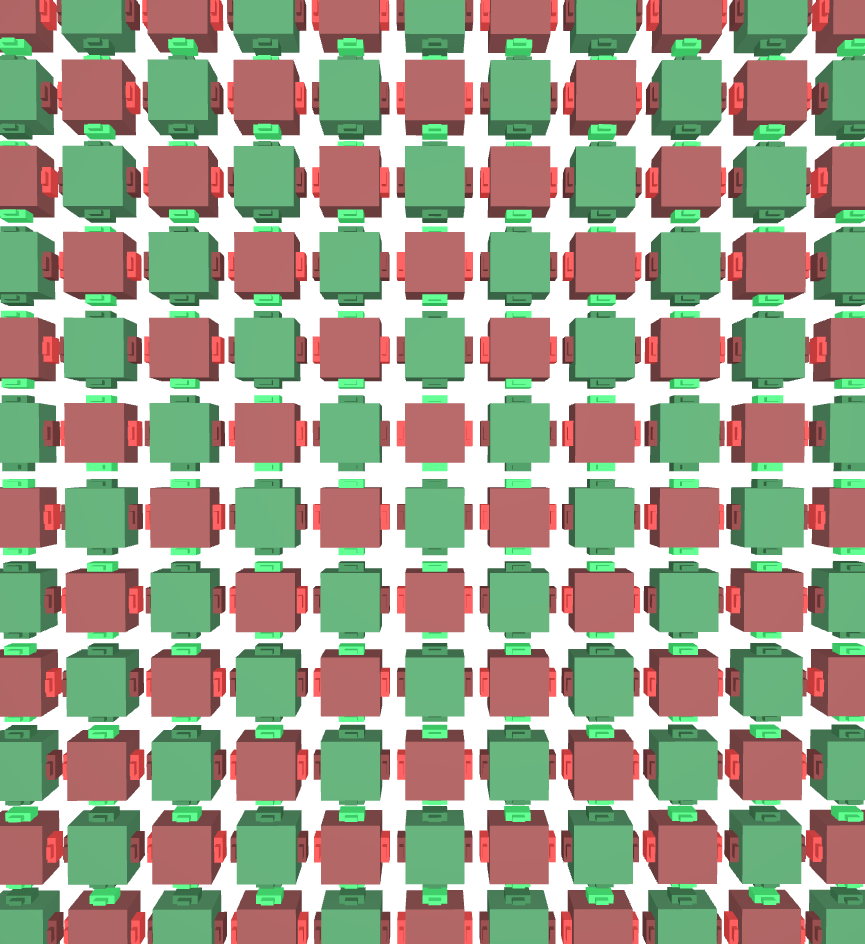
\includegraphics[width=0.6\textwidth]{figures/unbounded.png}
    \caption{Examples of undefined assemblies. a) Unbounded assembly that tiles the plane using two species \href{https://akodiat.github.io/polycubes?rule=05050a08000085858a880000}{05050a08000085858a880000}, b) An undeterminisic assembly of a ``giraffe duck'' with a neck that can have a new length each time it is assembled}
    \label{fig:sat_alg}
\end{figure}

\section{Example solves}

  